\section{Relativistic Heavy-Ion Collider (RHIC)}

The Relativistic Heavy Ion Collider (RHIC), at Brookhaven National Laboratory (BNL), is the only collider with dedicated running for heavy ion research (the CERN Large Hadron Collider runs heavy ions for only about one month per year), and the only polarized proton collider ever built. Two concentric accelerator rings 2.4 miles in circumference containing a total of 1,740 superconducting magnets afford RHIC the capability to independently accelerate and collide ion beam species from $\rm ^1_1H (p)$ to  $\rm ^{238}_{92}U$ at energies between 3.85 GeV and 254.9 GeV per nucleon and different spin polarizations for protons (\(p\)), as shown in \ref{fig:RHICSpecies}. These capabilities make RHIC the most flexible and capable collider in the world for transformative studies of extreme states of nuclear matter and the origin of the proton spin.

\begin{figure}[h]
	\label{fig:RHICSpecies}
	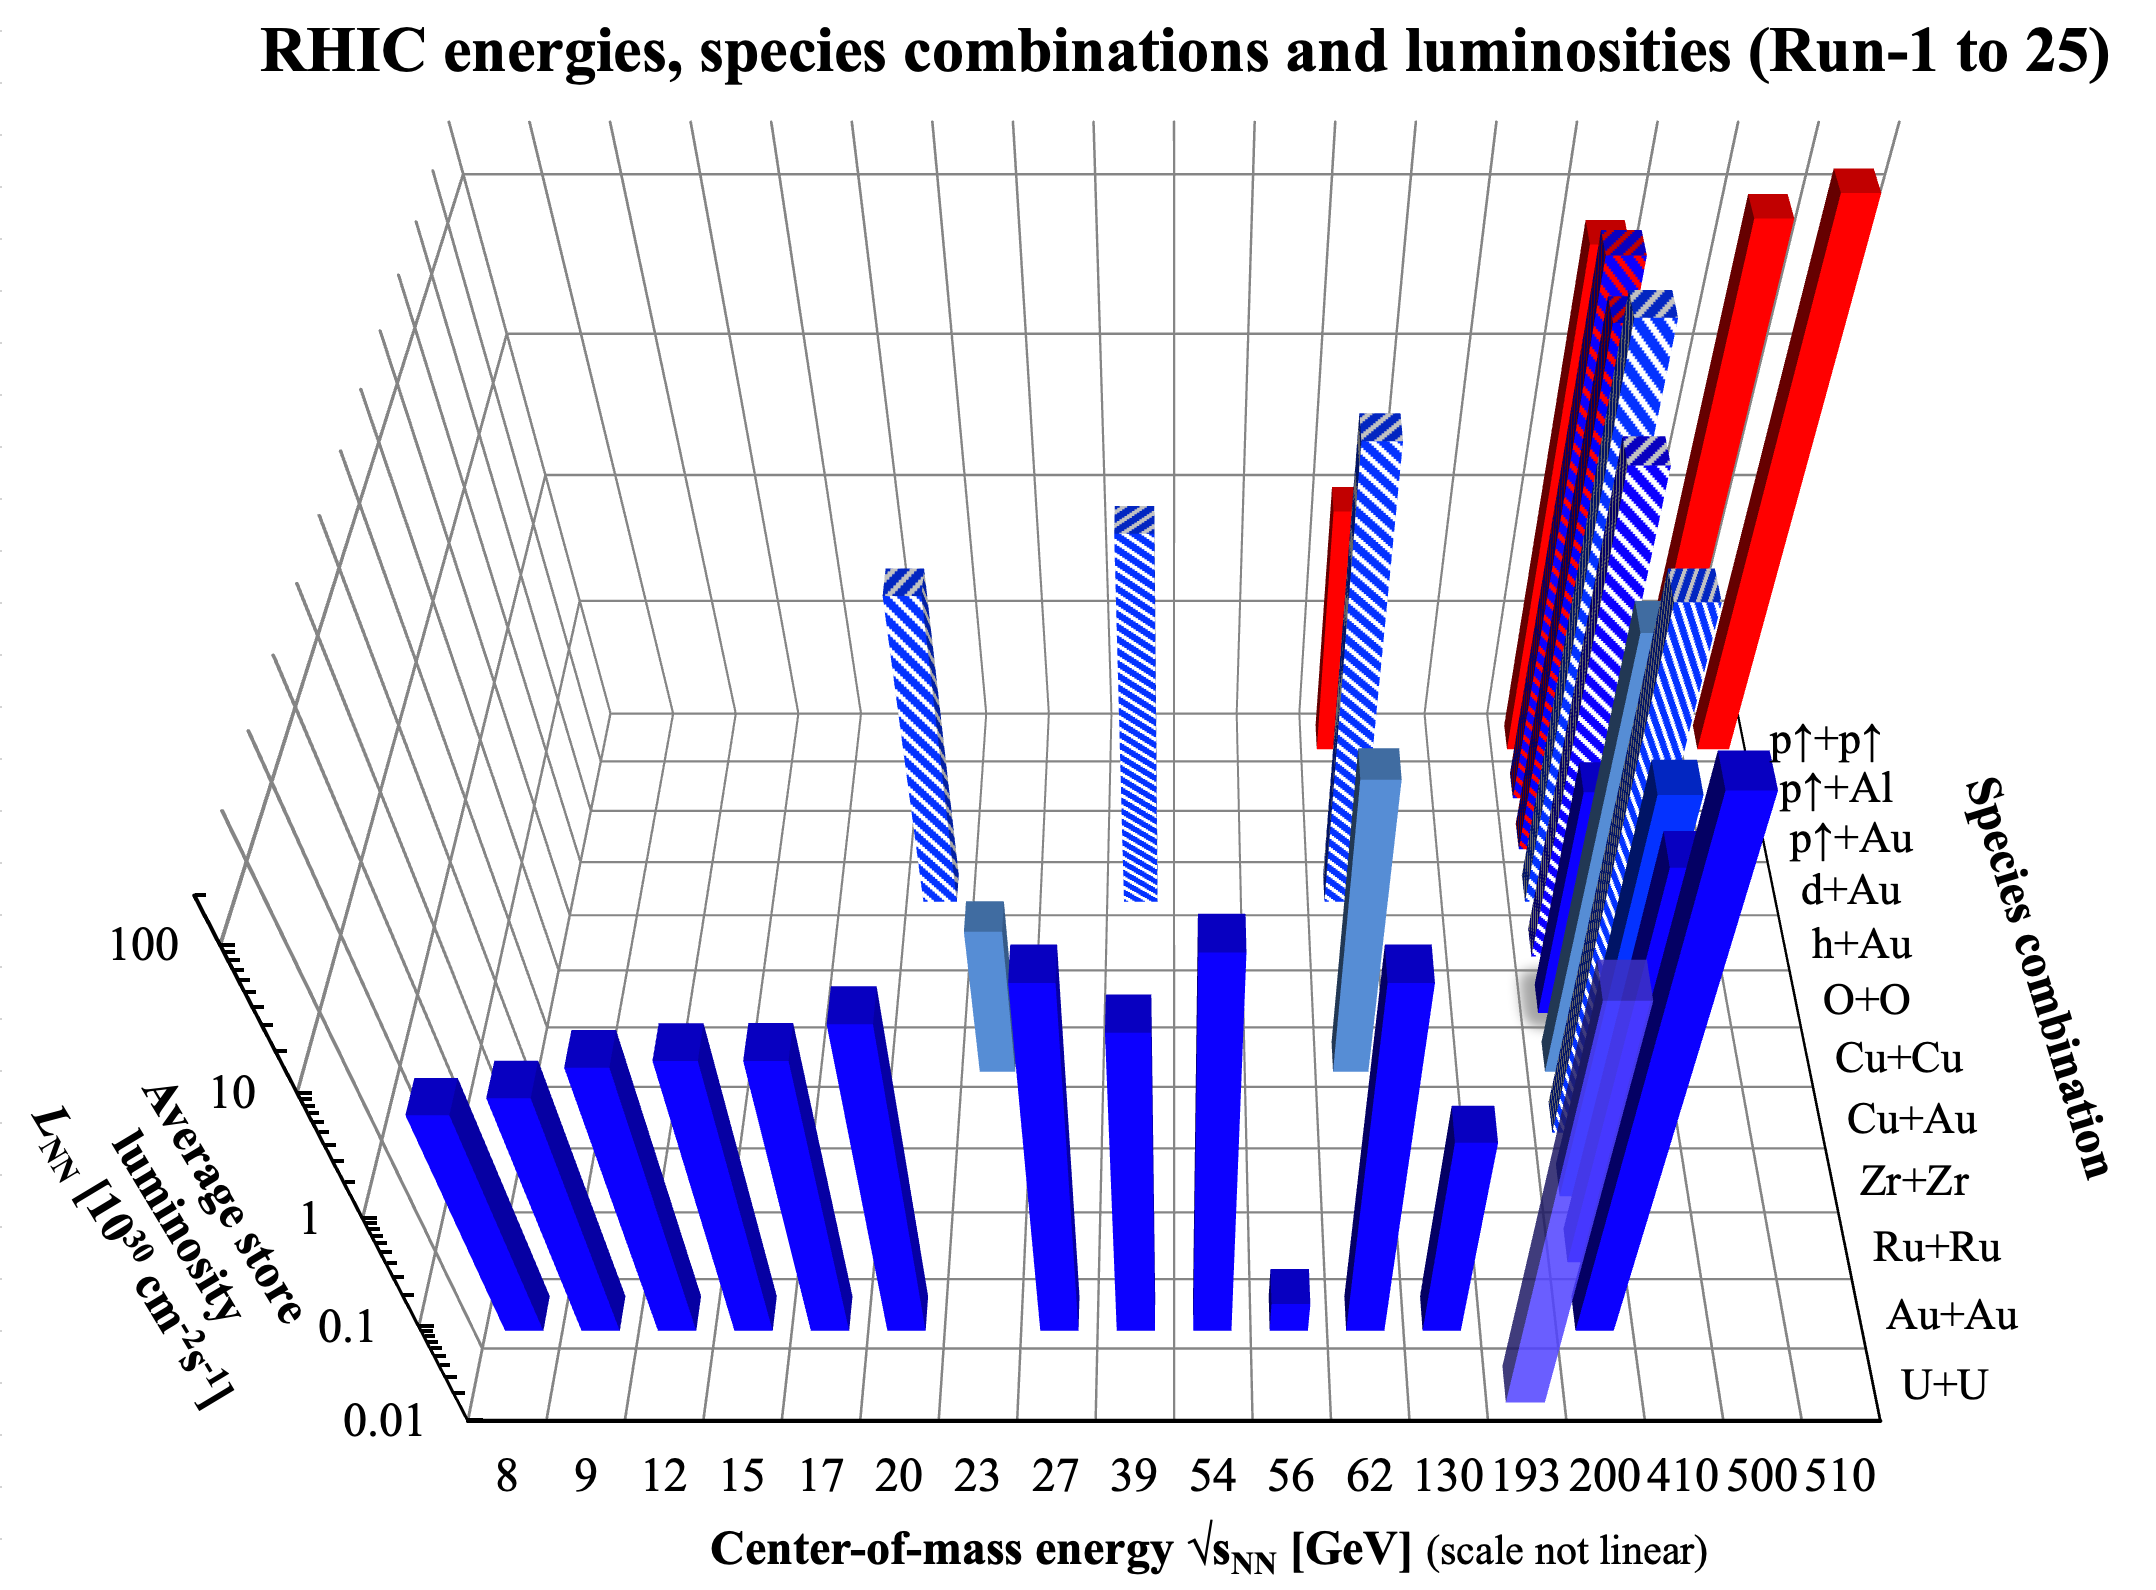
\includegraphics[width=\linewidth]{figures/RhicSpecies.png}
	\caption{Summary of RHIC energies, species combinations, and luminosities for runs between 2000 and 2026. Taken from \cite{RHICRunSummary}.}
\end{figure}
On February 6th 2026 RHIC ended operations with collisions of $\rm ^{16}_{8}O$ nuclei at \(\sqrt{s_\mathrm{NN}} = 200\)~GeV recorded by the \emph{Solenoidal Tracker At RHIC (STAR)} and \emph{sPHENIX} detectors. Over it's 25 years of active existence, it has performed \(\sim 300\)~trillion collisions of 49 unique pairs of nuclei, collected \(\sim 450\)~petabytes of data, whose analysis has led to over 650 publications. Eventually, one of RHIC’s ion storage rings will be removed and replaced with a new ring for storing accelerated electrons inside the existing accelerator tunnel, and the other major components of the RHIC accelerator complex will live on as parts of the upcoming Electron-Ion Collider (EIC).    
%\emph{strong Pioneering High Energy Nuclear Interaction eXperiment}.25 years. 

\begin{figure}[h]
	\label{fig:Final }
	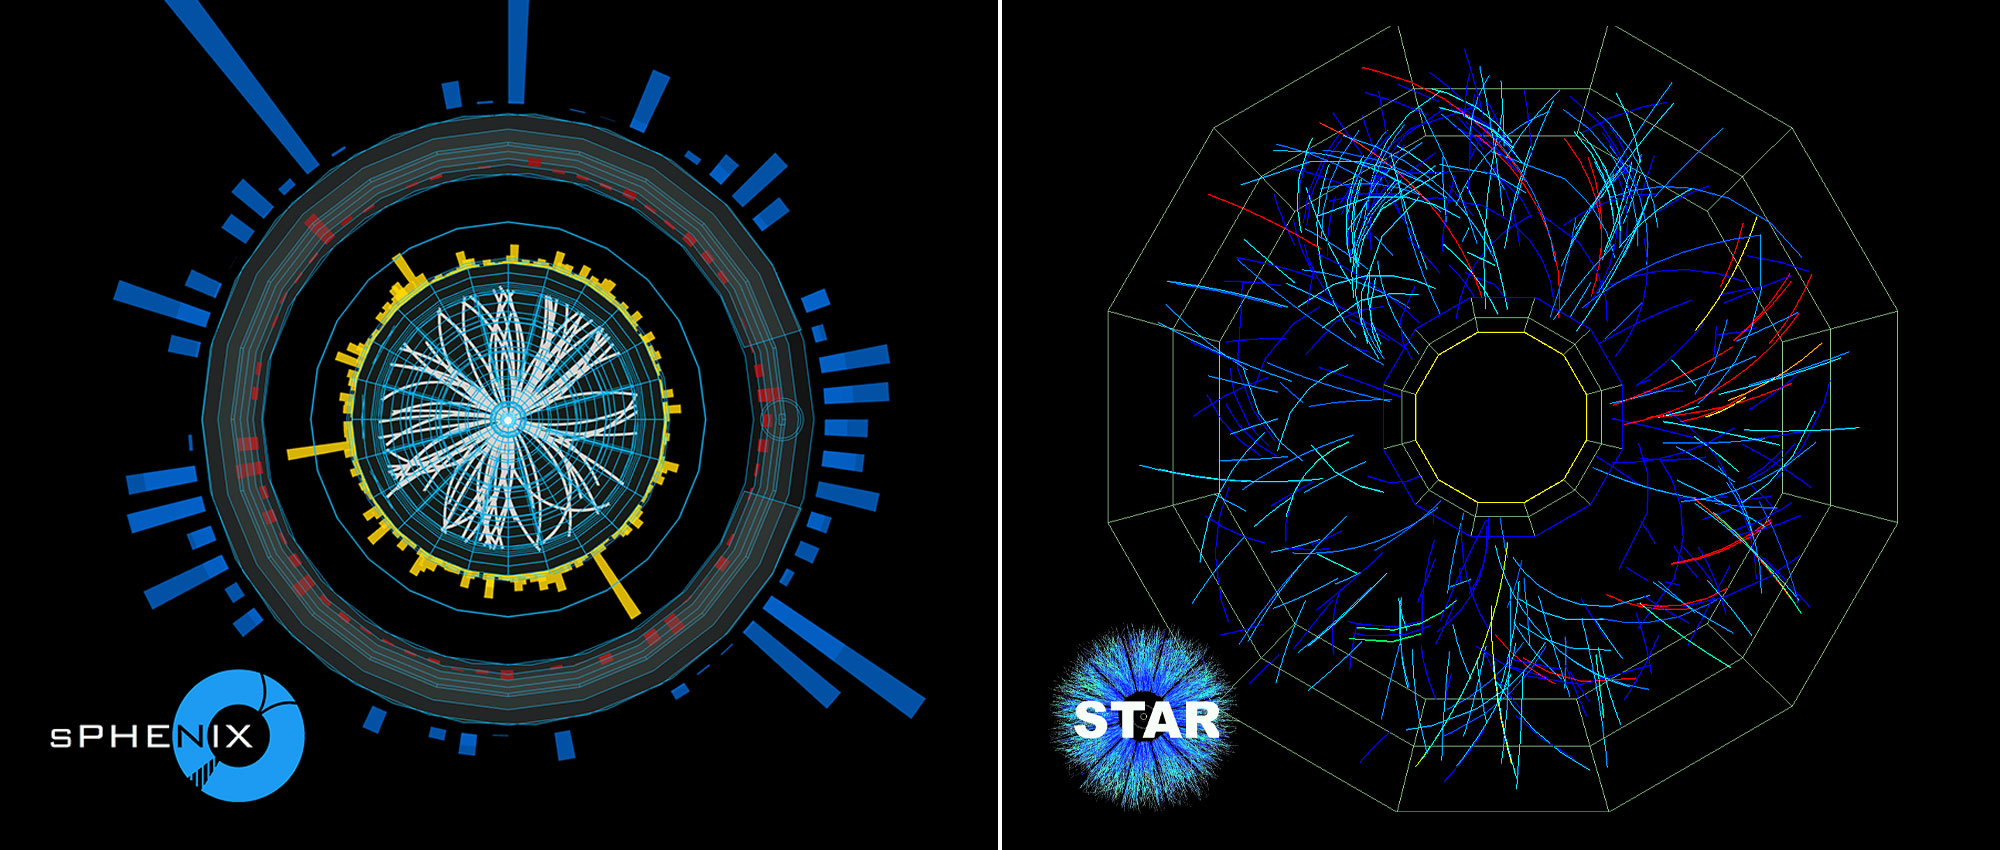
\includegraphics[width=\linewidth]{figures/sphenix-star-events-star-final-hr.jpg}
	\caption{Some of the final O+O collisions at \(\sqrt{s_\mathrm{NN}} = 200\)~GeV captured by the sPHENIX and STAR detectors at the RHIC. }
\end{figure}

\subsection{From stable matter to little bangs}
Before collisions, the nuclei have to be created first by taking the corresponding atoms and stripping off all their electrons. That process looks different for different nuclei. 

\begin{figure}[h]
		\centering
		\label{fig:RHIC-AGS }
		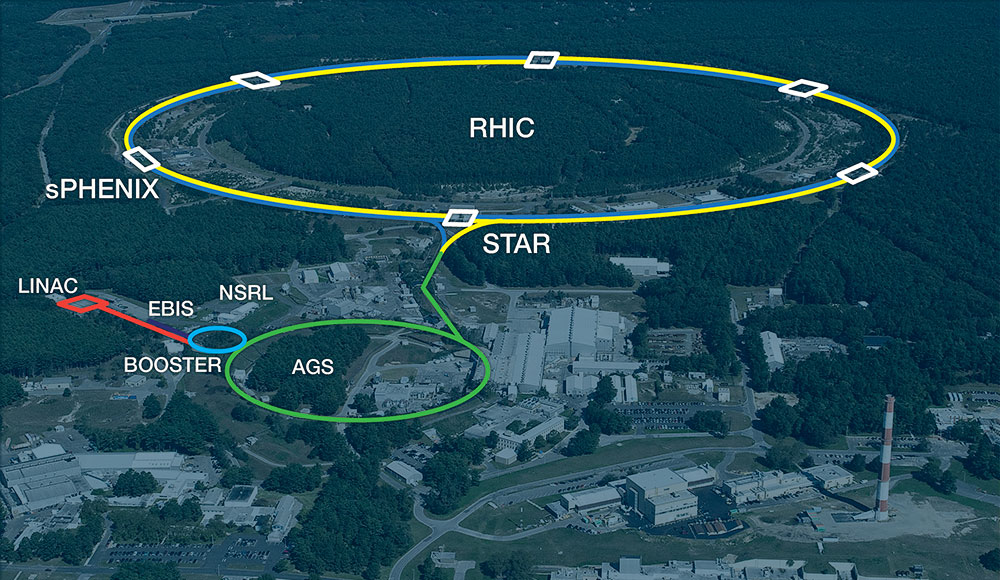
\includegraphics[width=0.6\linewidth]{figures/rhic-aerial-hr.jpg}
	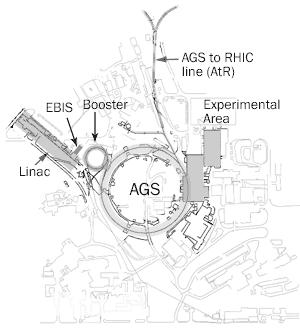
\includegraphics[width=0.3\linewidth]{figures/ags-complex}
	\caption{(Left) An aerial view of the Relativistic Heavy Ion Collider (RHIC), showing the locations of the facilities used for accelerating different ions, and the positions of the STAR and sPHENIX detectors. Taken from \cite{RHICRun23}.}
\end{figure}

\begin{itemize}
	\item \textbf{For protons} it is \emph{Optically Pumped Polarized \(H^-\) Ion Source (OPPIS)} fed into the \emph{Linear Accelerator (LINAC)}. The LINAC accelerates them to \(\sim 200\)~MeV and injects into the \emph{Booster Synchrotron} at which point, the two electrons are stripped away by a carbon foil. They are accelerated to upto 2.5 GeV and fed into the \emph{ Alternating Gradient Synchrotron (AGS)} which accelerates the proton beam to about 25 GeV.
	\item \textbf{For heavy-ions} like $\rm ^{197}_{79}Au$, a \emph{Laser Ion Source (LION)} extracts \(Au^+\) ions using laser ablation, which go into \emph{Electron Beam Ion Source (EBIS)} which ionizes them to \(Au^{32+}\) and accelerates them to 2 MeV per nucleon using electron beams.  Then they enter the booster synchrotron which accelerates them to about 95 MeV per nucleon. While exiting from the synchrotron, the atoms are stripped of more electrons by passing them through a stripping foil, and atoms in the $\rm Au^{77 + }$ state are fed to the AGS.  The beam's kinetic energy up to 8.86 GeV per nucleon for these Au atoms and the final two K shell electrons are stripped. 
	%Resulting beam of $\rm Au^{79 + }$ nuclei that are transported in the \emph{AtR (AGS-to-RHIC)} beampipe to the RHIC storage rings.
\end{itemize}
when the ion beam reached top speed in the AGS, it was taken down another beamline called the AGS-to-RHIC (AtR) transfer line. At the end of this line, a switching magnet sent the ion bunches down each of two beamlines to fill RHIC's two ion storage rings. Bunches directed left filled the clockwise RHIC ring (blue) while those directed right traveled counterclockwise in the second RHIC ring (yellow). In the rings, superconducting radio-frequency (RF) cavities accelerate the ion bunches to energies of 100 GeV per nucleon for heavy ions (255 GeV for protons), with four cavities operating at 28.15 MHz to generate standing waves of electric fields for the acceleration and ten 197 MHz cavities maintaining beam stability during storage. Superconducting dipole magnets with 3.5 T fields keep the beams on a circular path, while quadrupole magnets focus the ion beams. A total of 1,740 superconducting magnets are used in the two rings at RHIC, cooled by liquid Helium at $< 4.6$ K. An aerial view of the RHIC complex with the different subsystems is shown in Fig \ref{fig:RHIC-AGS}. 

There are 6 interaction regions (IR) around the RHIC complex, where the two beams cross and allow for detectors to be placed. 4 such detectors have existed during RHIC's operation: At 10 o'clock and 2 o'clock, the PHOBOS and BRAHMS experiments operated only for the first few years of RHIC (ending in 2006). At 8 o’clock, the PHENIX experiment collected data from 2000 to 2016 and was then transformed into the sPHENIX detector which began operations in 2023. STAR sits at the 6 o'clock position, and has been the only experiment running for all 25 years of RHIC's existence.

\section{Solenoidal Tracker at RHIC (STAR)}

\begin{figure}[h]
	\centering
	\label{fig:STARSchematic}
	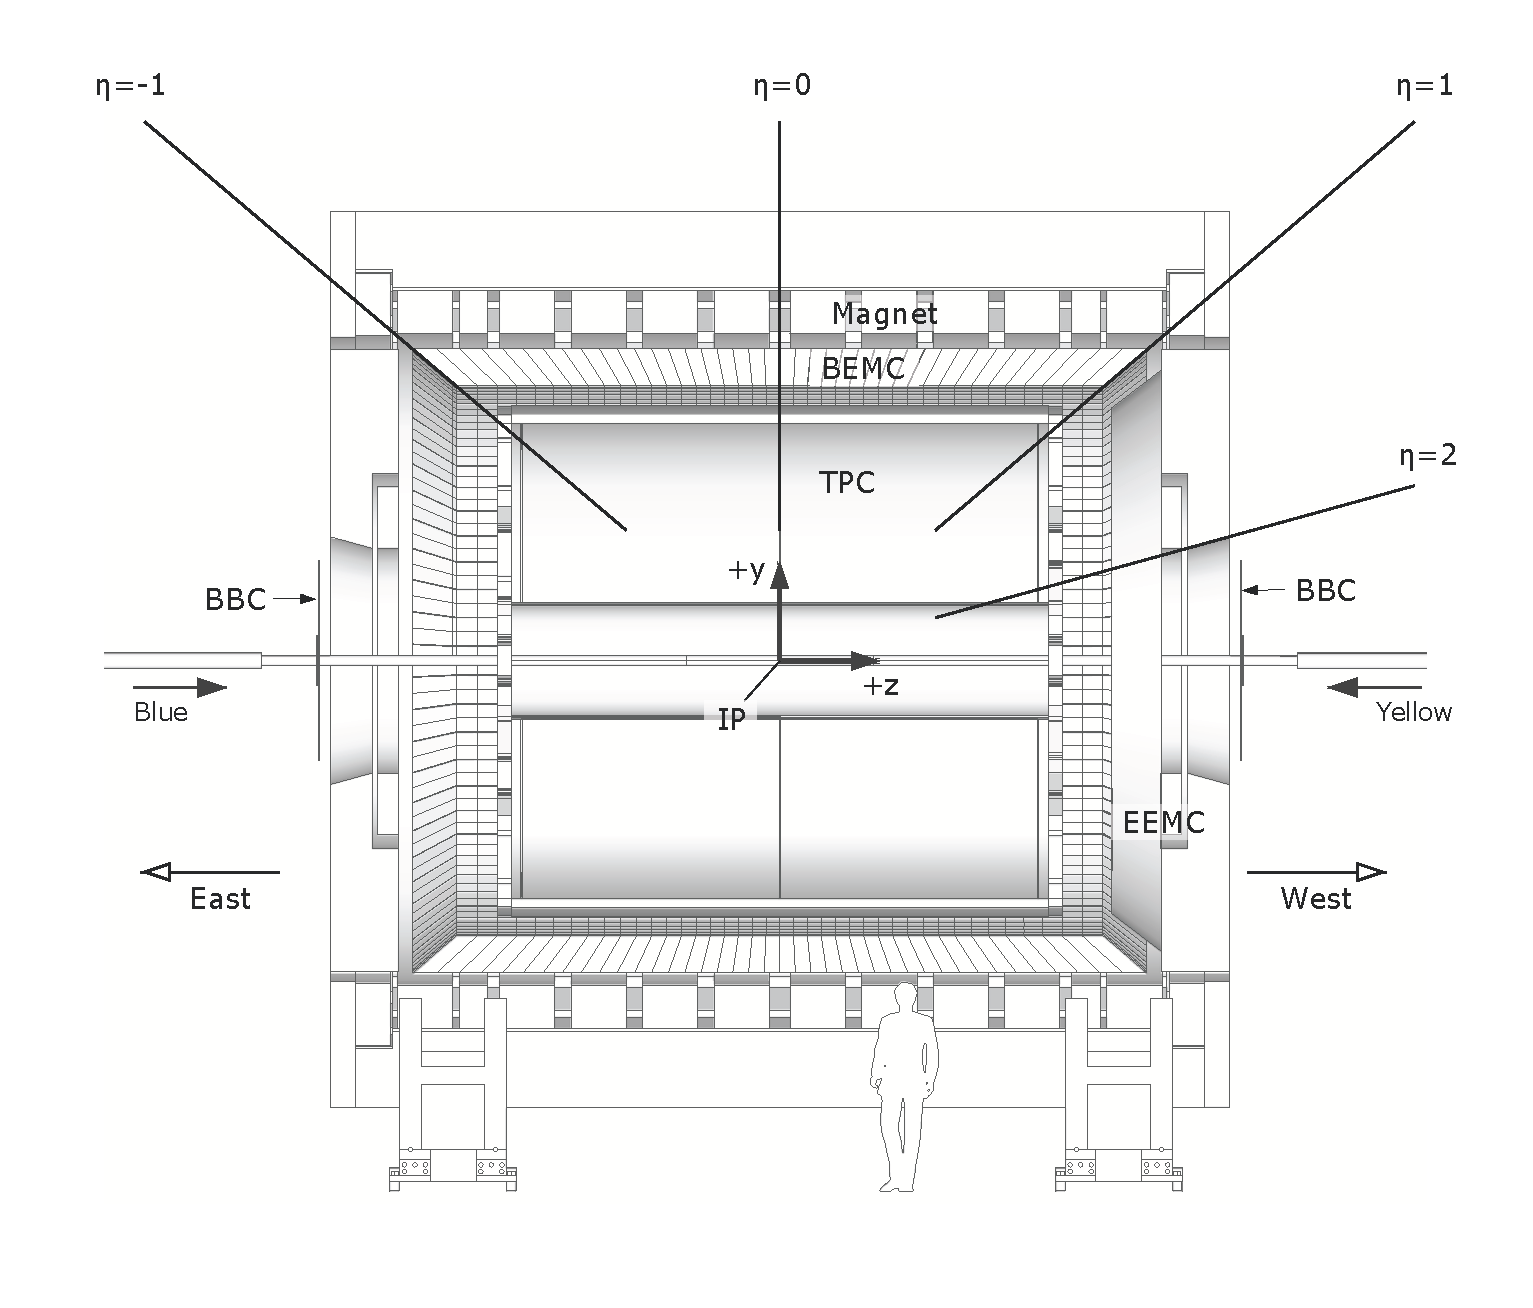
\includegraphics[width=0.8\linewidth]{figures/star_cutout.eps}
	\caption{Illustration of the STAR Coordinate System.}
\end{figure}